\documentclass[11pt,a4paper]{article}
\usepackage{fullpage}
\usepackage{tabu}
\usepackage[utf8]{inputenc}
\usepackage{tikz}
\usepackage{pgf}
\usetikzlibrary{arrows,automata}
\usetikzlibrary{positioning}
\title{Beastly Heis v1.0}
\author{Kolbjørn Austreng, Andreas Våge}

\tikzset{
    state/.style={
           rectangle,
           rounded corners,
           draw=black, very thick,
           minimum height=2em,
           inner sep=2pt,
           text centered,
           },
}

\begin{document}
\maketitle
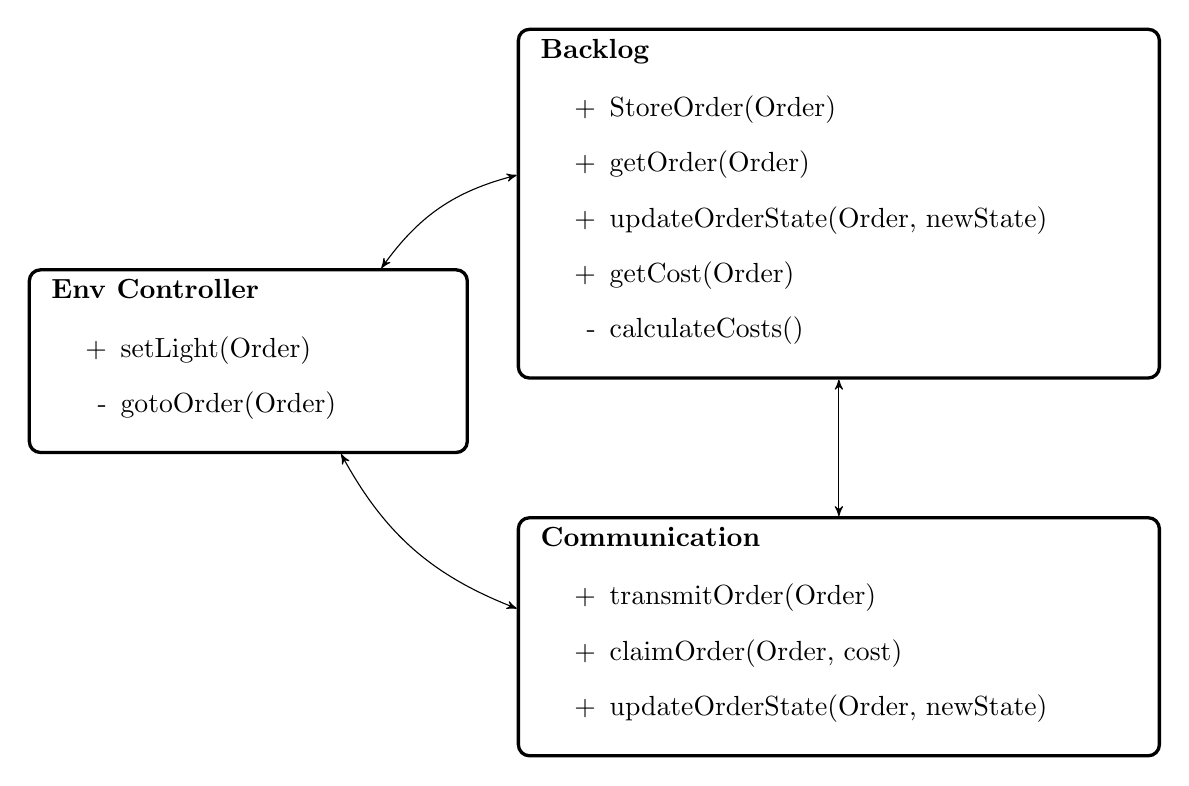
\begin{tikzpicture}[->,>=stealth']

 % Position of Env Controller 
 % Use previously defined 'state' as layout (see above)
 % use tabular for content to get columns/rows
 % parbox to limit width of the listing
 \node[state] (Env Controller) 
 {\begin{tabular}{l}
  \textbf{Env Controller}\\
  \parbox{5cm}{\begin{itemize}
   \item[+] setLight(Order)
   \item[-] gotoOrder(Order)
  \end{itemize}
  }
 \end{tabular}};

 \node[state,       % layout (defined above)
  text width=8cm,   % max text width
  yshift=2cm,       % move 2cm in y
  right of=Env Controller,   
  node distance=7.5cm,  
  anchor=center] (Backlog)  % posistion relative to the center of the 'box'
  {\begin{tabular}{l}
  \textbf{Backlog}\\
  \parbox{8cm}{\begin{itemize}
   \item[+] StoreOrder(Order)
   \item[+] getOrder(Order)
   \item[+] updateOrderState(Order, newState)
   \item[+] getCost(Order)
   \item[-] calculateCosts()

  \end{itemize}
  }
 \end{tabular}};
 
 % STATE Communication
 \node[state,
  below of=Backlog,
  yshift=-4.5cm,
  anchor=center,
  text width=8cm] (Communication) 
 {\begin{tabular}{l}
  \textbf{Communication}\\
  \parbox{8cm}{\begin{itemize}
   \item[+] transmitOrder(Order)
   \item[+] claimOrder(Order, cost)
   \item[+] updateOrderState(Order, newState)

  \end{itemize}
  }
 \end{tabular}};

 
 % draw the paths and and print some Text below/above the graph
 \path[<->] (Env Controller)  edge[bend left=20]   (Backlog)
 (Env Controller)        edge[bend right=20]  (Communication)
 %(Communication)     edge[loop below]    node[anchor=north,below]{$SC_n\neq 0$} (Communication)
 (Communication)     edge                 (Backlog);

\end{tikzpicture}
\section*{Oder object}
\begin{tabu}{|X|X|}
\hline
\textbf{Order} & Comment\\ \hline
+ type & Internal / External\\
+ floor & Destination floor\\
+ timestamp & Set by computer that first received order\\
+ origin IP & Set by computer that first received order\\
+ state & Queued, In progress, Timed out, Complete\\ \hline
\end{tabu}
\section*{Environment Controller}
\subsubsection*{+ setLight(Order)}
Sets the light corresponding to the floor of an Order object.
\subsubsection*{- gotoOrder(Order)}
Moves the elevator from its current position to the floor of an Order object.
\section*{Backlog}
\subsubsection*{+ storeOrder(Order) ok}
Saves an order from either \textit{Environment Controller} or \textit{Communications} to the backlog. Returns acknowledgement.
\subsubsection*{+ getOrder(Order) ok}
Returns to the \textit{Environment Controller} the next most feasible order. Returns acknowledgement if such an order exists, no-acknowledgement if there are no orders.
\subsubsection*{updateOrderState(Order, newState) ok}
Changes the state of an Order object. Returns acknowledgement.
\subsubsection*{+ getCost(Order) cost}
Returns the cost of taking a specific order for this elevator.
\subsubsection*{- calculateCosts()}
Calculates the costs of all the orders in the backlog for this elevator.
\section*{Communication}
\subsubsection*{+ transmitOrder(Order) ok}
Transmits an Order object to all the other nodes in the network. Acknowledges if at least one other elevator received the order transmit.
\subsubsection*{+ claimOrder(Order, cost) ok}
Attempts to claim an order in the backlog. Transmits own cost of taking on this order. Acknowledges if no other elevators have a lower cost on specified order.
\subsubsection*{+ updateOrderState(Order, newState) ok}
Broadcasts an order state update to ensure that the backlogs are identical.
\end{document}